\chapter{Конструкторская часть}
В этом разделе будут поставлены требования к ПО, привелены схемы реализаций алгоритмов,
а также описаны классы эквивалентности для функциональных тестов


\section{Требования к ПО}
Приведем список требований к ПО:

Требования к входным данным: матрица заполнена целыми числами; допускается, что один из линейных размеров матрицы может быть нулевым.

Требования к выводу:  программа должна выводить матрицу, получившуюся в результате умножения.

\section{Разработка алгоритмов}
На рисунке 2.1 приведена схема реализации алгоритма классического умножения матриц.
На рисунках 2.2 приведена схема реализации алгоритма Винограда.
На рисунке 2.3 приведена схема реализации оптимизированного алгоритма Винограда.

\FloatBarrier
\begin{figure}[hp]
	\begin{center}
		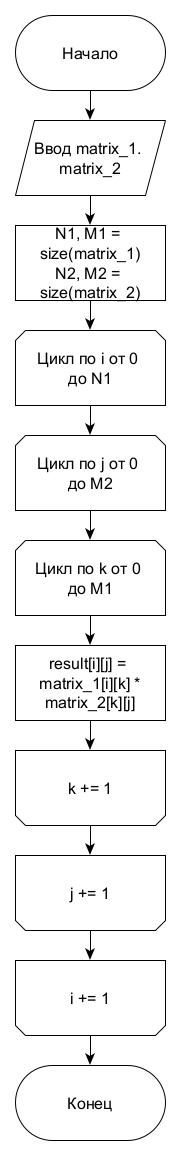
\includegraphics[height=23cm]{graph/classic.jpg}
	\end{center}
	\caption{Разработка алгоритма классического умножения матриц}
\end{figure}
\FloatBarrier

\FloatBarrier
\begin{figure}[hp]
	\begin{center}
		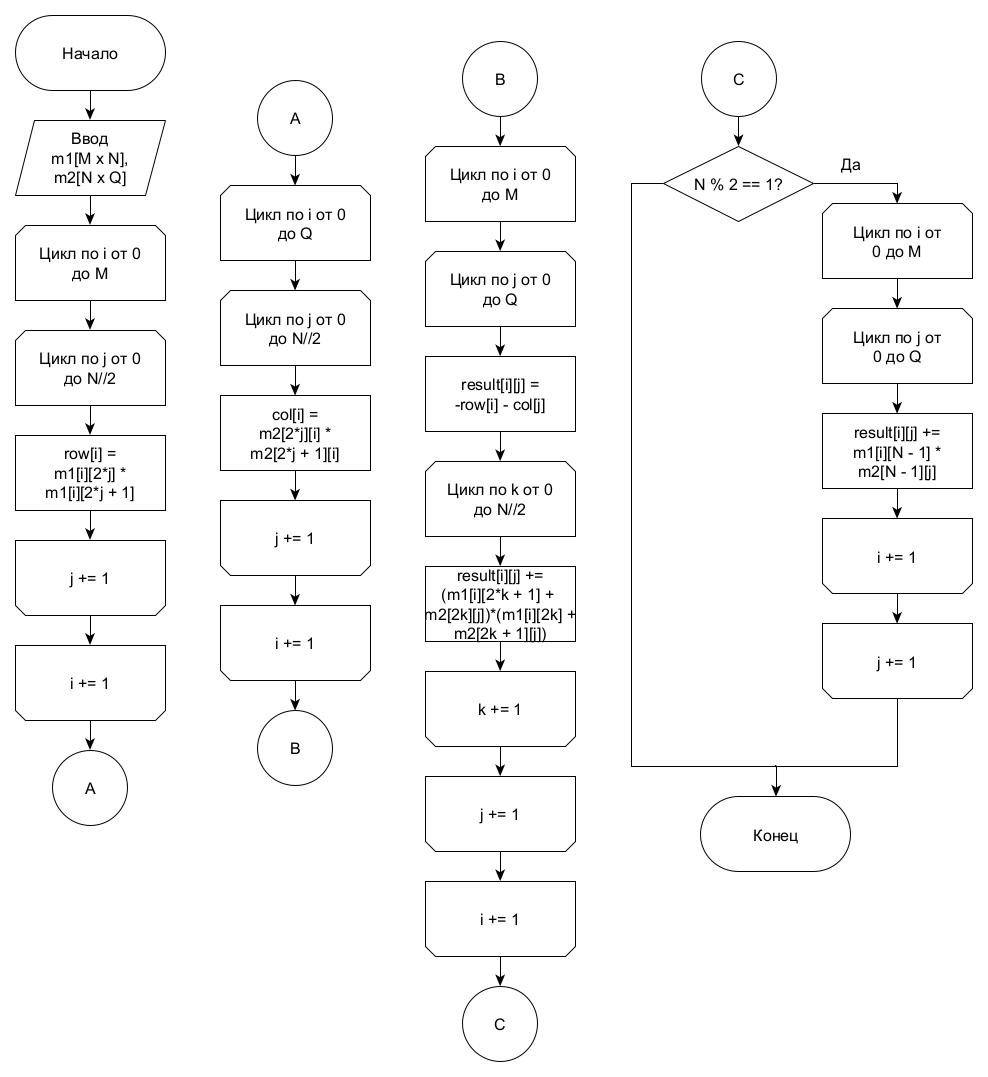
\includegraphics[width=\linewidth]{graph/vinograd.jpg}
	\end{center}
	\caption{Разработка алгоритма Винограда}
\end{figure}
\FloatBarrier

\FloatBarrier
\begin{figure}[hp]
	\begin{center}
		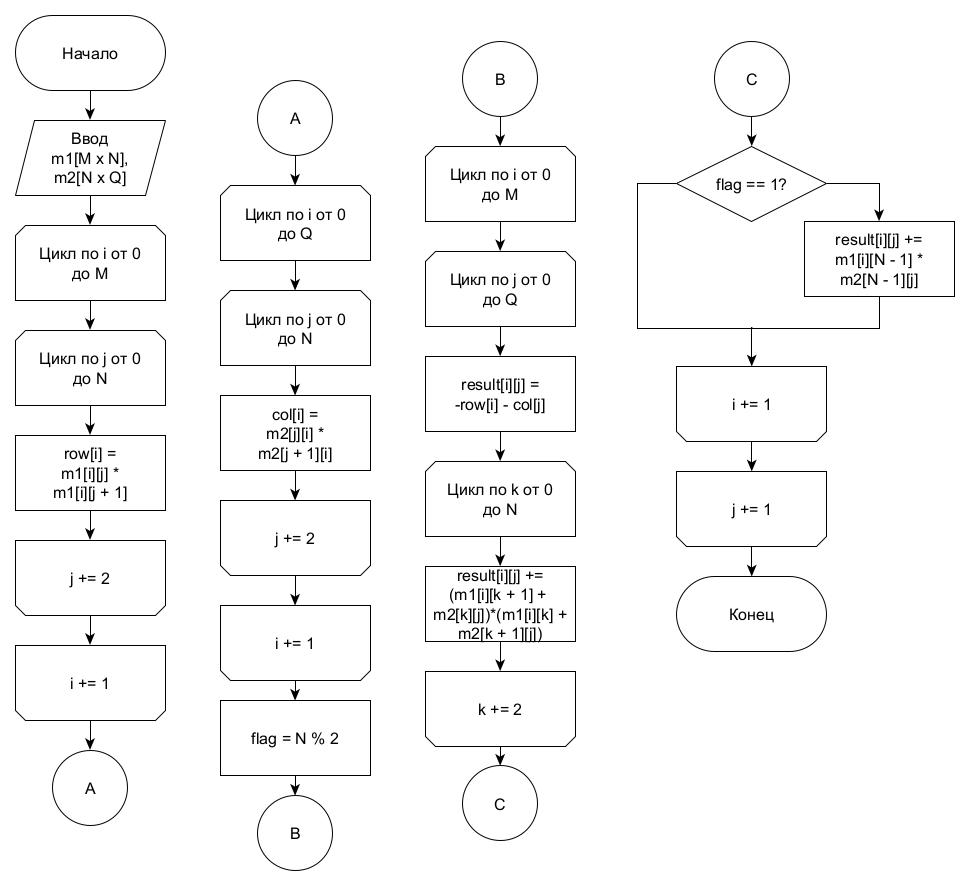
\includegraphics[width=\linewidth]{graph/optvinograd.jpg}
	\end{center}
	\caption{Схема оптимизированного алгоритма Винограда}
\end{figure}
\FloatBarrier

\section{Типы данных для алгоритмов}
Тестирование реализации алгоритмов будет производиться на целых числах, 
которые могут быть и отрицательными, и равны нулю. Несмотря на это,
сами реализации алгоритмов универсальны и предназначены для любых численных типов данных.

Размер матрицы может быть произвольным.

\section{Способ тестирования}
Для подхода к тестированию, был выбран метод черного ящика.
Выбор подхода может быть обусловлен следующей причиной:
реализаций алгоритмов требуется в первую очередь правильность работы.
Реализация сама по себе не требует тестировки, так как в точности
повторяет теоретические принципы, сформированные в аналитическом
разделе.

Классами эквивалентности были выбраны следующие сущности:
\begin{itemize}
	\item одна из матриц нулевого размера;
	\item матрицы не соответствуют друг другу по размеру;
	\item матрицы размером в $1 \times 1$;
	\item чётные размеры матрицы;
	\item нечётные размеры матрицы;
	\item одна из матриц - единичная;
	\item одна из матриц - нулевая.
\end{itemize}

Для корректного сравнения требуется для каждой реализации умножения матриц
сравнить полученный на выходе результат с эталонным.

\section*{Вывод}
Были приведены требования к ПО, схемы реализации алгоритмов.
Были определен способ тестирования алгоритмов.